\documentclass[fleqn]{article}
\usepackage[english]{babel}
\usepackage{amsmath}
\usepackage{amsthm}
\usepackage{graphicx}
\usepackage[utf8]{inputenc}

%%%%%%%% MARGIN
\usepackage[left=1in, right=1in, top=0.8in, bottom=0.8in]{geometry}

%%%%%%%% NO PARAGRAPH INDENT
% https://tex.stackexchange.com/questions/27802/set-noindent-for-entire-file
\setlength\parindent{0pt}

%%%%%%%% SUB-FIGURE PACKAGE
\usepackage{subcaption}

\usepackage{pdfpages}

%%%%%%%% HYPERREF PACKAGE
\usepackage{hyperref}
\hypersetup{linkcolor=blue}
\hypersetup{citecolor=blue}
\hypersetup{urlcolor=blue}
\hypersetup{colorlinks=true}

%%%%%%%% MULTI-COLUMNS PACKAGE
\usepackage{multicol}

%%%%%%%% SETS DEFINITIONS
\usepackage{amssymb}
%%%% Important sets
\renewcommand{\O}{\mathbb{O}}
\newcommand{\N}{\mathbb{N}}
\newcommand{\Z}{{\mathbb{Z}}}
\newcommand{\Q}{{\mathbb{Q}}}
\newcommand{\RR}{{\mathbb{R}}}

%%%% Statistics
\newcommand{\E}[1]{\mathbb{E}\left[#1 \right]}
\newcommand{\V}[1]{\mathbb{V}\left[#1 \right]}
\newcommand{\cov}[1]{\mathrm{Cov}\left[#1 \right]}

%%% Misc Math
% Spaces after/before left/right
\let\originalleft\left
\let\originalright\right
\renewcommand{\left}{\mathopen{}\mathclose\bgroup\originalleft}
\renewcommand{\right}{\aftergroup\egroup\originalright}

% Norm and abs
\newcommand{\norm}[1]{\left\lVert#1\right\rVert}
\newcommand{\abs}[1]{\left\lvert#1\right\rvert}

%%%% Superscript to the left
% https://latex.org/forum/viewtopic.php?t=455
\usepackage{tensor}
\newcommand{\app}[3]{\tensor*[^{#1}]{\left(#2, #3\right)}{}}


%%%%%%%% SPLIT EQUATIONS
% https://tex.stackexchange.com/questions/51682/is-it-possible-to-pagebreak-aligned-equations
\allowdisplaybreaks

%%%%%%%% CODE RENDERING
% Compile with flag -shell-escape
\usepackage{minted}

%%%%%%%% EXAM PACKAGE
\usepackage{mathexam}

%%%%%%%% CHANGE MARGINS ITEMIZE
\usepackage{enumitem}

%%%%%%%% START DOCUMENT

\ExamClass{EC0301 - Time Series}
\ExamName{Assignment \#8}
\ExamHead{\today}

\let\ds\displaystyle

\begin{document}
 \vspace{0.3cm}
   % Information of the student
   \begin{itemize}[leftmargin=6.25cm, labelsep=0.5cm]

     \item[\textit{Name}] \scalebox{1.2}{David Plazas Escudero} % Name
     \item[\textit{Student code}] 201710005101 % Code

   \end{itemize}
\vspace{0.3cm}

% Each of the items to solve
\begin{enumerate}
    \item \textit{Using the dataset from the class, select a city different from Medellín and estimate the model proposed by auto.arima for the variable in levels and for the variable transformed by Box-Cox. Verify if these models satisfy the validation assumptions and estimate the predictions for next year. Do you think that, given the current situation, these predictions are realistic?}
    
    The libraries and the data input for this assignment is presented as follows:
    \begin{minted}{R}
    library(readxl)
    library(MASS)
    library(timeSeries)
    library(tseries)
    library(tidyverse)
    library(forecast)
    library(fUnitRoots)
    library(feasts)
    
    Inflacion <- read_excel("1.2.4.IPC_Por ciudad_IQY.xlsx", skip=1044)

    Inflacion <- Inflacion %>%
                 select(Cali) %>%
                 mutate(Cali = as.numeric(Cali)) %>%
                 na.omit()
    
    Cali <- ts(Inflacion$Cali,
                   start = c(1979,12),
                   end = c(2020,9),
                   frequency = 12)
    \end{minted}
    
    The plot of the complete time series data is presented in Figure \ref{fig:TSComplete}.
    
    \begin{minted}{R}
    plot(Cali)
    \end{minted}
    \begin{figure}[H]
        \centering
        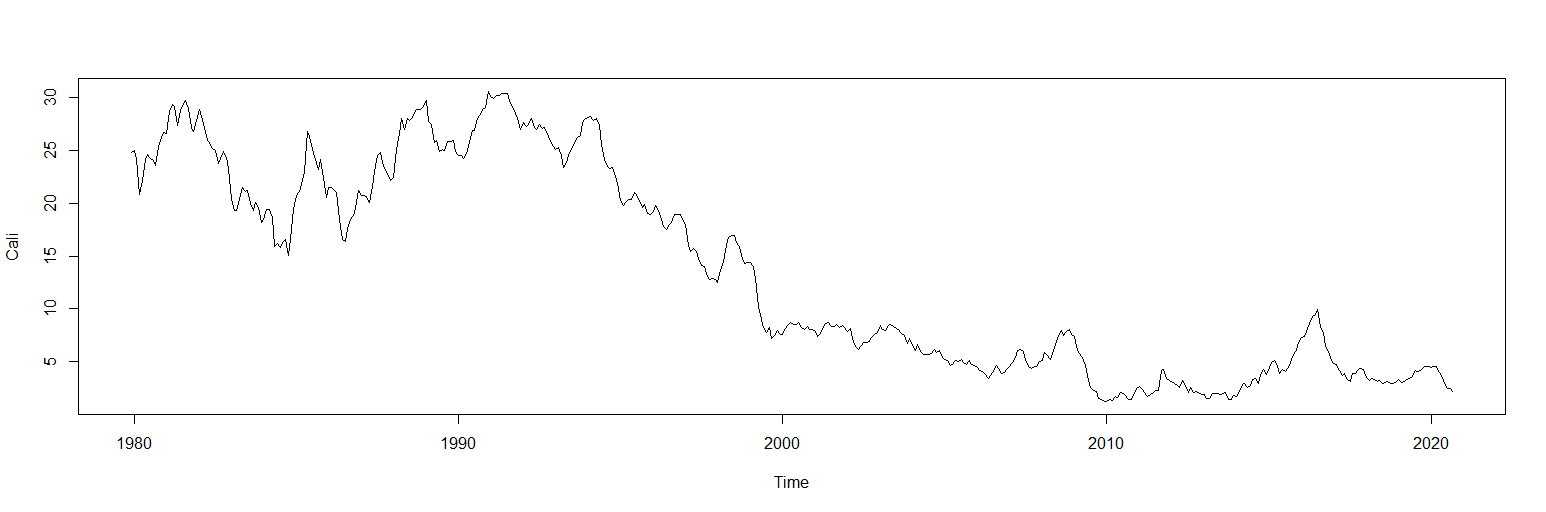
\includegraphics[width=\linewidth]{figs/TSComplete.png}
        \caption{Time series data.}
        \label{fig:TSComplete}
    \end{figure}
    Note that the D.G.P. of the time series before the year 2000 is different from the one after 2000. This is due to changes in law and policies in Colombia. The data will then be considered only after the year 2000. Hence, the time series data considered is presented in Figure \ref{fig:TSCut}.
    \begin{minted}{R}
    Cali <- window(Cali, start = c(2000,1), end=c(2020,9))
    plot(Cali)
    \end{minted}
    \begin{figure}[H]
        \centering
        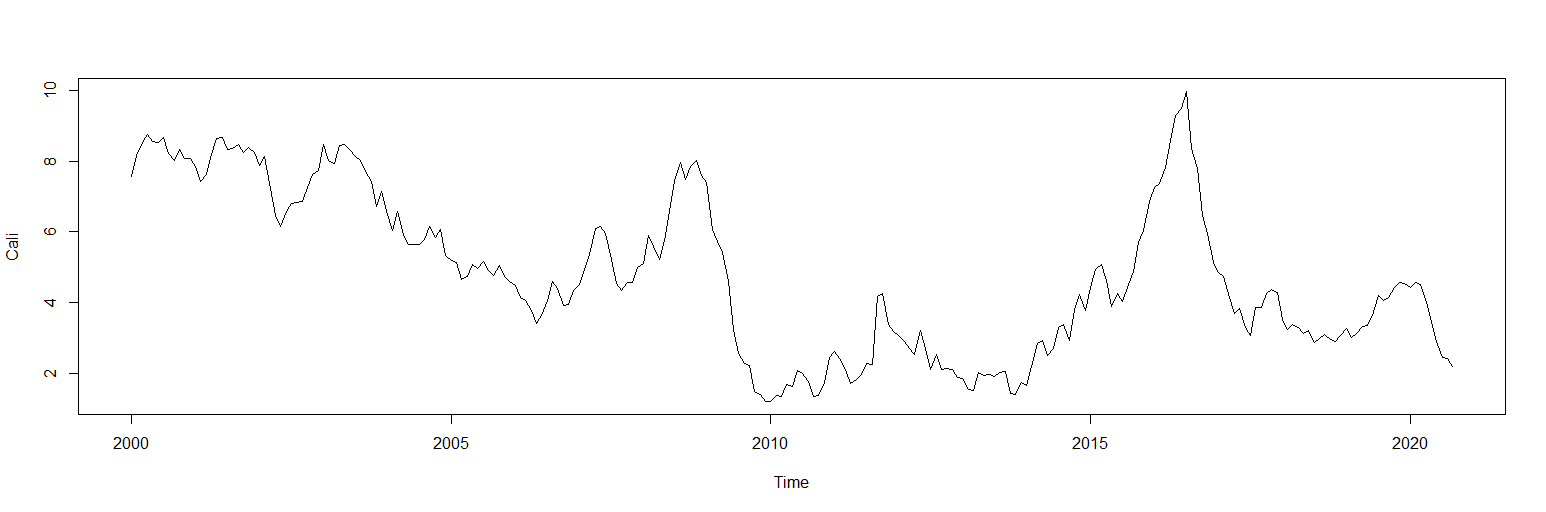
\includegraphics[width=\linewidth]{figs/TSCut.png}
        \caption{Reduced time series data.}
        \label{fig:TSCut}
    \end{figure}
    Now, this time series data is transformed using Box-Cox. This transformation yielded a value of $\lambda=0.4646$. The code for this transformation and the new transformed data is:
    \begin{minted}{R}
    bc <- boxcox(Cali ~ 1)
    (lambda <- bc$x[which.max(bc$y)])
    Cali_bc <- BoxCox(Cali, lambda)
    plot(Cali_bc)
    \end{minted}
    The obtained $\lambda$ and the transformed time series data are presented in Figures \ref{fig:cox} and \ref{fig:TSCox}, respectively.
    \begin{figure}[H]
        \centering
        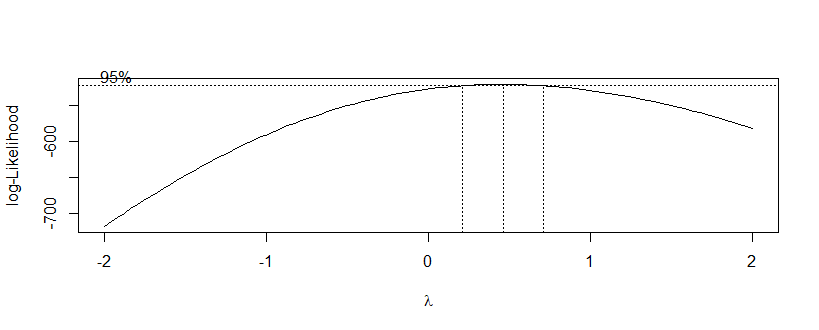
\includegraphics[width=\linewidth]{figs/cox.png}
        \caption{Box-Cox $\lambda$.}
        \label{fig:cox}
    \end{figure}
    \begin{figure}[H]
        \centering
        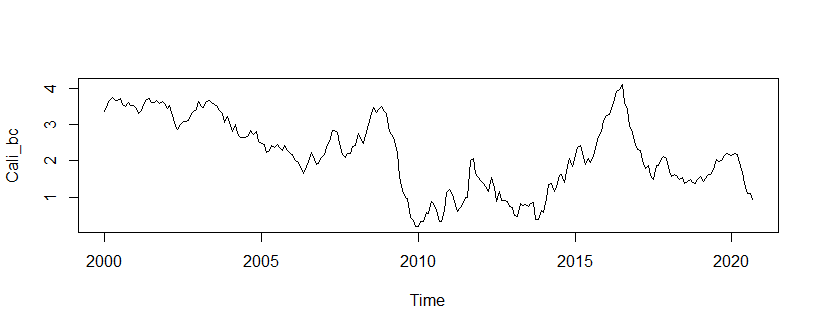
\includegraphics[width=\linewidth]{figs/TSCox.png}
        \caption{Box-Cox transformed time series.}
        \label{fig:TSCox}
    \end{figure}
    Note that the variance of the time series was significantly reduced. For the ARIMA estimation, the order of differentiation will be first calculated. The time series data (and the data transformed by Box-Cox) was tested first for stationarity, using the Augmented Dickey-Fuller, Phillips-Perron and KPSS tests. All tests indicated that the original data (and the one resulting of Box-Cox) is not stationary; these result can be verified using the following code:
    \begin{minted}{R}
    unitrootTest(Cali)
    unitrootTest(Cali_bc)
    pp.test(Cali)
    pp.test(Cali_bc)
    kpss.test(Cali)
    kpss.test(Cali_bc)
    \end{minted}
    However, after taking one difference on the data, all tests passed for stationarity of the data. These can be concluded from the following code:
    \begin{minted}{R}
    diff_cali <- diff(Cali)
    diff_cali_bc <- diff(Cali_bc)
    
    unitrootTest(diff_cali) 
    unitrootTest(diff_cali_bc) 
    pp.test(diff_cali) 
    pp.test(diff_cali_bc) 
    kpss.test(diff_cali) 
    kpss.test(diff_cali_bc) 
    \end{minted}
    Therefore, for both the original and transformed data, the $d$ order in the ARIMA($p,d,q$) will be assumed as 1, and the 2 models were estimated with this hypothesis. One model is for the original data, and the other for the transformed data by Box-Cox.
    
    The partial autocorrelation plot for both datasets are presented in Figures \ref{fig:PACFCut} and \ref{fig:PACFCox}. Note that both plots show that there exists an significant autocorrelation in the 12th lag in both plots.
    \begin{minted}{R}
    pacf(Cali)
    pacf(Cali_bc)
    \end{minted}
    \begin{figure}[H]
        \centering
        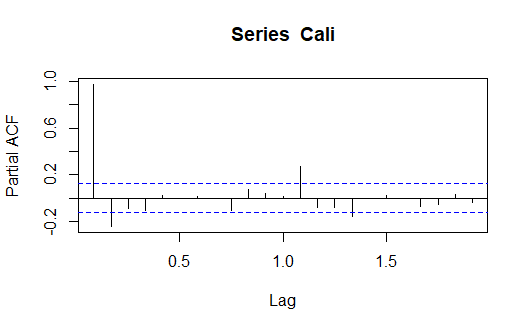
\includegraphics[width=0.6\linewidth]{figs/PACFCut.png}
        \caption{PACF of time series data.}
        \label{fig:PACFCut}
    \end{figure}
    \begin{figure}[H]
        \centering
        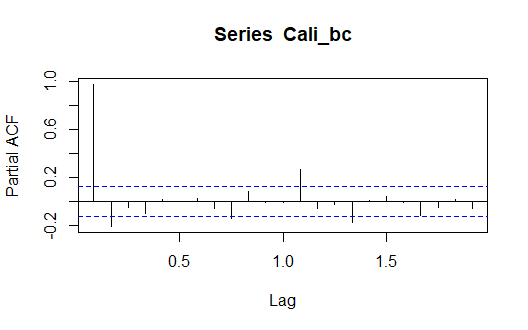
\includegraphics[width=0.6\linewidth]{figs/PACFCox.png}
        \caption{PACF of transformed time series data.}
        \label{fig:PACFCox}
    \end{figure}
    Based on the determination of $d$, and given that the data is autocorrelated in the 12th lag, the estimated models were obtained using the following commands:
    \begin{minted}{R}
    # first model
    modelo1 <- auto.arima(Cali, max.p = 12, max.q = 12, d=1,
                      seasonal = FALSE)
    # second model
    modelo2 <- auto.arima(Cali_bc, max.p = 12, max.q = 12, d=1,
                      seasonal = FALSE)
    \end{minted}
    The result for the first model is an ARIMA(1,1,0) and for the second one is an ARIMA(2,1,2). The verification of the validation assumptions will be now performed for both models:
    \begin{itemize}
        \item \textbf{White-Noise Residuals:} The mean of the estimated residuals for both models were $-0.01599$ and $-0.0004$, which are both really close to 0. The variance seems to stay constant over time, from the residuals plots in Figure \ref{fig:mod1res} and \ref{fig:mod2res}.
        \begin{minted}{R}
        # first model
        mean(modelo1$residuals)
        plot(modelo1$residuals)
        acf(modelo1$residuals)
        pacf(modelo1$residuals)
        
        # second model
        mean(modelo2$residuals)
        plot(modelo2$residuals)
        acf(modelo2$residuals)
        pacf(modelo2$residuals)
        \end{minted}
        \begin{figure}[H]
        \centering
        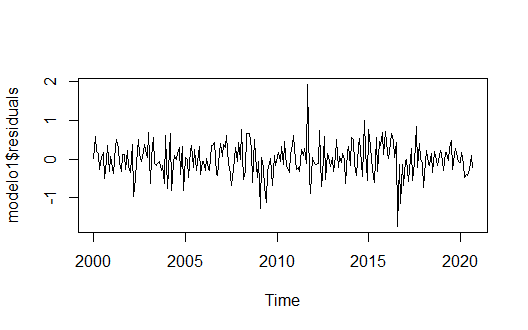
\includegraphics[width=0.75\linewidth]{figs/mod1res.png}
        \caption{Residuals of first model.}
        \label{fig:mod1res}
        \end{figure}
        \begin{figure}[H]
        \centering
        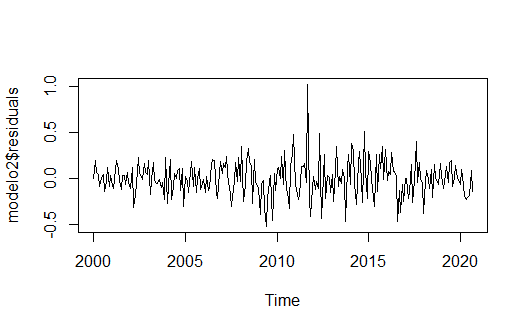
\includegraphics[width=0.75\linewidth]{figs/mod2res.png}
        \caption{Residuals of second model.}
        \label{fig:mod2res}
        \end{figure}
        
        Now, in order to state that the residuals are, indeed, white-noise, the autocorrelations must be calculated. The ACF and PACF of the first model are respectively presented in Figures \ref{fig:ACFmod1res} and \ref{fig:PACFmod1res}, note that the residuals seem to be still autocorrelated.
        \begin{figure}[H]
        \centering
        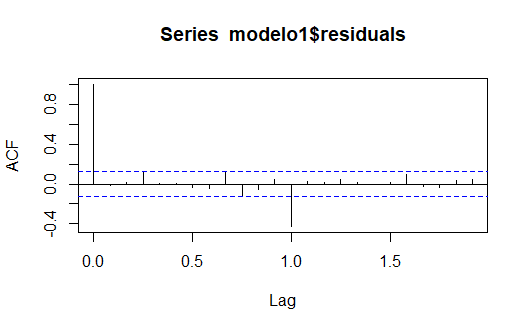
\includegraphics[width=0.75\linewidth]{figs/ACFmod1res.png}
        \caption{ACF of residuals of first model.}
        \label{fig:ACFmod1res}
        \end{figure}
        \begin{figure}[H]
        \centering
        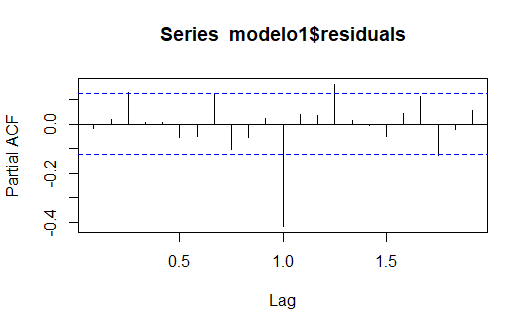
\includegraphics[width=0.75\linewidth]{figs/PACFmod1res.png}
        \caption{PACF of residuals of first model.}
        \label{fig:PACFmod1res}
        \end{figure}
        
        The ACF and PACF of the second model are respectively presented in Figures \ref{fig:ACFmod2res} and \ref{fig:PACFmod2res}, note that the residuals seem to be still autocorrelated.
        \begin{figure}[H]
        \centering
        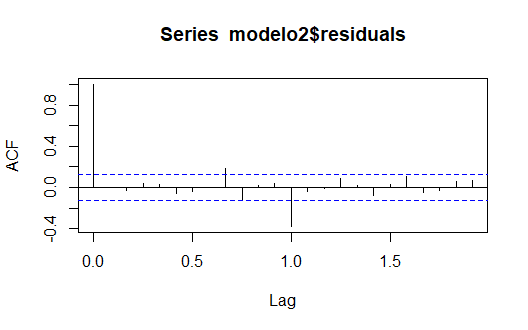
\includegraphics[width=0.75\linewidth]{figs/ACFmod2res.png}
        \caption{ACF of residuals of second model.}
        \label{fig:ACFmod2res}
        \end{figure}
        \begin{figure}[H]
        \centering
        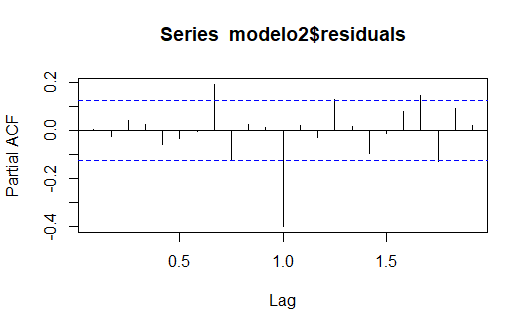
\includegraphics[width=0.75\linewidth]{figs/PACFmod2res.png}
        \caption{PACF of residuals of second model.}
        \label{fig:PACFmod2res}
        \end{figure}
        This was better tested using the Ljung-Box test for autocorrelation, through the following commands:
        \begin{minted}{R}
        Box.test(modelo2$residuals, lag=12, type = "Ljung", fitdf = 4)
        Box.test(modelo1$residuals, lag=12, type = "Ljung", fitdf = 4)
        \end{minted}
        and in both cases, the null hypothesis of no autocorrelation was rejected. Hence, there is evidence of autocorrelation in the residuals. Then, they are not white-noise.
        \item \textbf{Stationarity and Invertibility:}
        \begin{minted}{R}
        plot(modelo1)
        plot(modelo2)
        \end{minted}
        \begin{figure}[H]
        \centering
        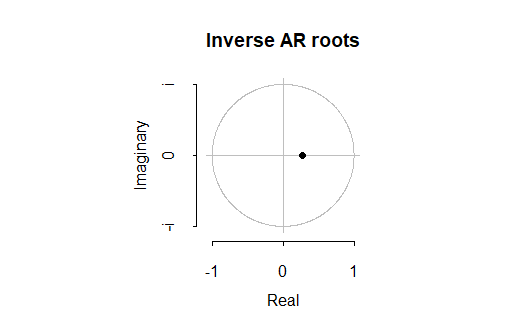
\includegraphics[width=0.75\linewidth]{figs/mod1roots.png}
        \caption{Roots of first model.}
        \label{fig:mod1roots}
        \end{figure}
        \begin{figure}[H]
        \centering
        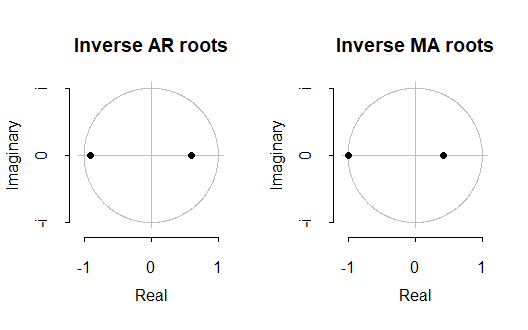
\includegraphics[width=0.75\linewidth]{figs/mod2roots.png}
        \caption{Roots of second model.}
        \label{fig:mod2roots}
        \end{figure}
        In this case, both models are stationary. The first model is invertible, since it does not have MA component. The second model is not invertible, since it appears that one of the roots is lying exactly in the unit circle.
        \item \textbf{Significant and Non-correlated Coefficients:} For the first model, the correlation between coefficients does not apply, since there is only one parameter. For the second model, the autocorrelation matrix is presented in Figure \ref{fig:mod2corr}. Note that all parameters are highly correlated.
        \begin{minted}{R}
        cov2cor(modelo2$var.coef)
        \end{minted}
        
        \begin{figure}[H]
        \centering
        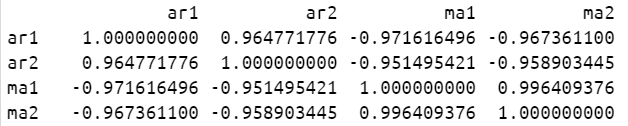
\includegraphics[width=0.75\linewidth]{figs/mod2corr.png}
        \caption{Correlation between coefficients of second model.}
        \label{fig:mod2corr}
        \end{figure}
        
        The significance was tested using a t-test with each parameter divided by its standard error. If this value is greater than 1.96, we say that the parameter is significant. For the first model, the parameter is significant. For the second model, not all parameters were significant.
        \begin{minted}{R}
        # first model
        (modelo1$coef)/sqrt(modelo1$var.coef) > 1.96
        # second model
        for (i in 1:4) {
          print((modelo2$coef[i])/sqrt(modelo2$var.coef[i,i]) > 1.96)
        }
        \end{minted}
        \item \textbf{D.G.P. representation:} To test that the model adequately represents the D.G.P., the White test for linearity was used in both models
        \begin{minted}{R}
        # first model
        white.test(Cali)
        # second model
        white.test(Cali_bc)
        \end{minted}
        The results for the tests show that the null hypothesis of linearity is not rejected. There is evidence of linearity in the series data for both models.
        \item \textbf{Goodness-of-fit:} In both cases, the models have a good fit to the data, with $R^2$ values of 0.9641 and 0.9619 respectively.
        \begin{minted}{R}
        # first model
        1 - modelo1$sigma2/var(Cali_bc)
        # second model
        1 - modelo2$sigma2/var(Cali_bc)
        \end{minted}
    \end{itemize}
    The prediction to one year was performed using the following code:
    \begin{minted}{R}
    h <- 12

    pred_modelo1 <- forecast(modelo1, h) 
    pred_modelo2 <- forecast(modelo2, h)
    
    pred_modelo2_corregido <- InvBoxCox(pred_modelo2$mean, lambda,
                                          biasadj = TRUE,
                                          fvar = var(Cali_bc))
    
    Data_pred <- data.frame(cbind(pred_modelo1$mean,
                                  pred_modelo2_corregido))
    Data_pred <- Data_pred %>%
                 mutate(t=seq(from = as.Date("2020/10/31"), 
                              to = as.Date("2021/09/30"), 
                              length.out = 12))
    
    ggplot(Data_pred) +
      geom_line(aes(x=t, y = pred_modelo1.mean,
                    colour = "Lineal"), size = 1) +
      geom_line(aes(x=t, y = pred_modelo2_corregido,
                    colour = "Box-Cox"), size = 1) +
      scale_colour_manual("", 
                          breaks = c( "Lineal",  "Box-Cox"),
                          values = c("red", "blue")) +
      theme_minimal()
    \end{minted}
    and the results are presented in Figure \ref{fig:preds}.
    
    \begin{figure}[H]
    \centering
    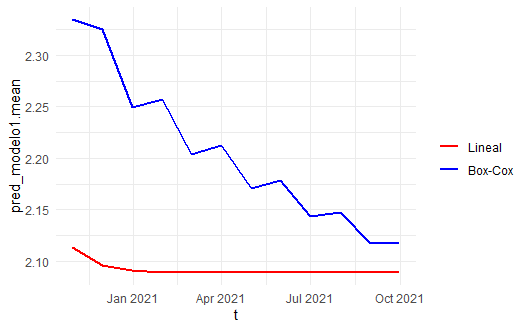
\includegraphics[width=0.75\linewidth]{figs/preds.png}
    \caption{Models predictions for 1 year.}
    \label{fig:preds}
    \end{figure}
    Given the current situation around the world, the predictions for the next months (or even years) cannot be completely reliable, since the current pandemic is an exogenous situation that has affected economy all around the world. In order to give reliable predictions, the time series data must include more data after this year, since we do not know yet if the D.G.P. or the trend has changed.
    
\end{enumerate}
\end{document}
